%\settikzpagecorners

In this section, we discuss how matrices are created, referenced and used in calculations.

\section{Matlab: Matrices}\label{sec:Matlab_matrices}

Each variable in Matlab is stored as a \textbf{matrix}, which is an array of numbers arranged in a rectangle of m rows and n columns.
One says that such a matrix is an m by n matrix, written as m $\times$ n.
A \textbf{vector} is any matrix that has either only one row (a ``row vector'') or one column (a ``column vector'').  A scalar, or number, is stored as a matrix that has exactly one row and one column (i.e, a $1 \times 1$ matrix).

\index{Matlab!Matrix Definition}

Let's look at some examples of how matrices are entered in Matlab.  Each matrix is enclosed in the symbols \cour{[} and \cour{]}, each comma (or space) separates entries on the same row and each semicolon indicates a new row.\\

\example{ex_label}{\po\\
\\
\cour{>> A = [1,2,3,4;5,6,7,8]} (or \cour{A = [1 2 3 4;5 6 7 8]})\\
\\
gives the $2 \times 4$ matrix\\
\\
\cour{A =}\\
\cour{\ps 1 2 3 4}\\
\cour{\ps 5 6 7 8}\\
\\
and\\
\\
\cour{>> B = [1; 6; 0; 9]}\\ 
\\
gives the $4 \times 1$ matrix\\
\\
\cour{B =}\\
\cour{\ps 1}\\
\cour{\ps 6}\\
\cour{\ps 0}\\
\cour{\ps 9}\\
\\
and\\
\\
\cour{>> C=[3]}\\ 
\\
gives the $1 \times 1$ matrix (i.e. a scalar)\\
\\
\cour{C =}\\
\cour{\ps 3}
}\\

\index{Matlab!semicolon (;)}
You may have noticed that the semicolon is used in a new way in the last example.  It is perhaps unfortunate, but there are symbols that are reused throughout Matlab code (including the semicolon, colon and comma) and the meaning of a particular symbol will depend on context.  Semicolons are used {\it inside} matrix definitions to indicate a new row while semicolons are used at the end of a line to suppress output.  Let's look at a few more examples.\\

\index{Matlab!colon (:)}
\example{ex_label2}{\po\\
\\
Suppose we wanted a matrix with the values 1 through 19 in a single (row) vector.  We could enter this as\\
\\
\cour{>> M = [1 2 3 4 5 6 7 8 9 10 11 12 13 14 15 16 17 18 19]}\\
\\
although this takes a little while to type (what if we wanted 1 to 1000?!).  Instead we use the \textbf{colon operator}.  The syntax to create this same matrix of 1 to 19 is shortened to\\
\\
\cour{>> M = [1:19]}.
}\\

In the last example, we can think of the colon as a ``range operator.''  Note that Matlab also accepts the slightly shorter \cour{M = 1:19} as well, which will be useful when we come to loops. In fact, the colon is more flexible (pun intended?) as we see in the next example.\\  

\example{ex_a}{\po\\
\\
The matrix defined as\\
\\
\cour{>> N = [1:2:19]}\\ 
\\
is the same as if we typed\\
\\
\cour{>> N = [1 3 5 7 9 11 13 15 17 19]}.
}\\

What is going on in this example?  Well, the general form in using two colons this way is \\

\cour{start value : step size : end value}\\

In \cour{N}, the 2 means to simply count ``by twos'' starting at 1 and ending at 19.  There's a slight limitation in that if we tried 
\cour{P = [1:2:20]} we would also get \cour{P} to equal \cour{[1 3 5 7 9 11 13 15 17 19]}.  Where's the 20?  Well, the syntax of \cour{start:step:end} actually means to begin at \cour{start}, add the \cour{step} one at a time and then stop at the point where adding one more step size would take us past the \cour{end} value.  So, in the matrix \cour{P}, we have to stop at 19 since adding two more would take us to 21 (past the \cour{end} value of 20).  But, suppose we actually wanted to end exactly at your last value?  That's where we use the command \cour{linspace} instead.\\
\index{Matlab Functions!\cour{linspace}}

\example{ex_linspace}{\po\\
\\
\cour{>> P = linspace(1,6,4)}\\  

Here we get\\
\\
\cour{P =}\\
\cour{\ps 1.0000    2.6667    4.3333    6.0000}\\

You can see that we started at 1 and ended at 6 and have 4 total values.  That's the exact syntax:\\

\cour{linspace(start,end,number of values)}
}\\

There are two special matrices that come up a lot too:\\

\index{Matlab Functions!\cour{ones}}
\index{Matlab Functions!\cour{zeros}}
\example{ex_zeroone}{\po\\
\\
\cour{>> G = ones(3,4)}\\ 
\\
gives the $3 \times 4$ matrix of all ones:\\
\\
\cour{G =}\\
\cour{\ps 1 1 1 1}\\
\cour{\ps 1 1 1 1}\\
\cour{\ps 1 1 1 1}\\
\\
\cour{>> H = zeros(2,5)}\\ 
\\
gives the $2 \times 5$ matrix of all zeros:\\
\\
\cour{H =}\\
\cour{\ps 0 0 0 0 0}\\
\cour{\ps 0 0 0 0 0}
}

\section{Matlab: Using Matrices}\label{sec:Matlab_using_matrices}

Let's look at how we can reference parts of a matrix.\\

\example{ex_matrixreference}{\po\\

Consider the matrix \cour{A = [1 2 3 4;5 6 7 8]}.  There are actually two ways to view this matrix, either as a rectangular array of 2 rows and 4 columns, or as a list of 8 elements.  Suppose we wanted to isolate the 7 in the matrix \cour{A} and store it as the variable \cour{temp}.  First, we can think of the 7 as being located in the second row and third column.  In this case, we can type:\\
\\
\cour{>> A = [1 2 3 4;5 6 7 8];}\\
\cour{>> temp = A(2,3)}\\
\\
with the result being:\\
\\
\cour{temp =}\\
\cour{\ps 7}\\

Second, we can think of 7 as being one of the eight elements total.  But, it is crucial to realize that we count elements in this way using a ``column precedence.''  This means that we count, one at a time, down the columns.  This means that we can think of 7 as being located in the 6th entry, or:\\
\\
\cour{>> temp = A(6)}\\
\\
also gives the result:\\
\\
\cour{temp =}\\
\cour{\ps 7}
}\\

For completeness, in the last example, if we think of \cour{A} as a matrix:\\
\\
\cour{A(1,1) = 1} \quad \cour{A(1,2) = 2} \quad \cour{A(1,3) = 3} \quad \cour{A(1,4) = 4} \\
\cour{A(2,1) = 5} \quad \cour{A(2,2) = 6} \quad \cour{A(2,3) = 7} \quad \cour{A(2,4) = 8} \\
\\
or, thinking of \cour{A} as a vector:\\
\\
\cour{A(1) = 1} \quad \cour{A(3) = 2} \quad \cour{A(5) = 3} \quad \cour{A(7) = 4} \\
\cour{A(2) = 5} \quad \cour{A(4) = 6} \quad \cour{A(6) = 7} \quad \cour{A(8) = 8} \\

If we wanted to store the entire first row of \cour{A} in the variable \cour{firstrow}, we would say that we want ``all four columns of the first row.''  This suggests that we can use the colon operator to shorten our work.  Namely,\\
\\
\cour{>> firstrow = A(1,1:4)}\\
\\
which gives\\
\\
\cour{firstrow =}\\
\cour{\ps 1 2 3 4}\\

But, there's an even shorter way to do this! If the colon doesn't have a start and end value, it simply lists all possible values!  Namely,\\
\\
\cour{>> firstrow = A(1,:)}\\
\\
also gives\\
\\
\cour{firstrow =}\\
\cour{\ps 1 2 3 4}\\

Ok, now what if we wanted the first row, but not the element in the first column?  There are two ways to do this.
First, we can use the colon as:\\
\\
\cour{>> mostoffirstrow = A(1,2:4)}\\
\\
which gives\\
\\\cour{mostoffirstrow =}\\
\cour{\ps 2 3 4}\\
\\
But, what if the matrix changes and we don't know how big \cour{A} has changed to?  Those sneaky programmers at Mathworks have a work around:\\
\\
\cour{>> mostoffirstrow = A(1,2:end)}\\
\\
also gives\\
\\
\cour{mostoffirstrow =}\\
\cour{\ps 2 3 4}

\section{Matlab: Matrix Operations}\label{sec:Matlab_matrix_operations}

Here we will explore the algebra of matrices.  It would be wise for the reader to have a basic knowledge of matrix algebra (or even linear algebra), but we will try and give plenty of explanatory examples.

\index{Matlab!dot operations ($.*, ./, .\wedge$)}
Just as for scalars, many of the common algebraic operations apply to matrices.  The symbols $+$ and $-$ carry over quite nicely in ``element-by-element'' operations as one would expect (or at least hope for).  Similarly, if you want element-by-element multiplication, division, or even exponentiation, these are given by $.*, ./$ and $.\wedge$ (yes, those each have a preceeding period and are pronounced \textbf{``dot times''},\textbf{ ``dot divide''} and \textbf{``dot exponent''}).  
Operations like ``regular'' multiplication, division, exponents, etc. have a very different meaning than one who hasn't been exposed to linear algebra might expect.  We also have operations like the matrix transpose.

Let's look at some examples using the matrices \cour{A = [1 2 3 4;5 6 7 8]} and \cour{B = [1; 6; 0; 9]}.
Again,\\
\\
\cour{A =}\\
\cour{\ps 1 2 3 4}\\
\cour{\ps 5 6 7 8}\\
and\\
\cour{B =}\\
\cour{\ps 1}\\
\cour{\ps 6}\\
\cour{\ps 0}\\
\cour{\ps 9}\\

\example{ex_scalarmultiplication}{\textbf{Scalar Multiplication}\\

Here we show how to multiply every entry in a matrix by a scalar:\\
\\
\cour{>> A = [1 2 3 4;5 6 7 8];3*A}\\ 
\\
gives\\
\\
\cour{ans =}\\
\cour{\ps \po 3  \po 6  \po 9 12}\\
\cour{\ps 15 18 21 24}
}
\po \\

One special operation for matrices is the matrix \textbf{transpose}, given by either \cour{transpose(A)} or the shorter \cour{A}\textquotesingle.  The transpose of a matrix is another matrix with the rows and columns interchanged.\\

\example{ex_transpose}{\textbf{Transpose}\\

\noindent\cour{>> A = [1 2 3 4;5 6 7 8];A}\textquotesingle\\
\\
\cour{ans =}\\
\cour{\ps 1 \, 5}\\
\cour{\ps 2 \, 6}\\
\cour{\ps 3 \, 7}\\
\cour{\ps 4 \, 8}\\
\\
and\\
\\
\cour{>> B = [1; 6; 0; 9];B}\textquotesingle\\
\\
\cour{ans =}\\
\cour{\ps 1 6 0 9} 
}\\

The example \cour{A}$\wedge 2$ gives an error saying \cour{A} must be square (here it is good to know some linear algebra), but \cour{A}$.\wedge 2$ gives element-by-element squaring:\\

\example{ex_elementsquare}{\textbf{Element by element squaring}\\
\\
\cour{>> A = [1 2 3 4;5 6 7 8];A}$. \wedge 2$\\
\\
\cour{ans = }\\
\cour{\ps \po 1 \po 4 \po 9 16}\\
\cour{\ps 25 36 49 64}
}
\po \\

Finally, we can create ``block'' matrices from smaller matrices by treating them as elements themselves and using the comma (or space) and the semicolon to create rows and columns.  We just have to make sure the dimensions of the matrices line up properly.  For example, we can stack two matrices.\\

\index{Matlab!Block Matrices}
\example{ex_stackmatrices}{\textbf{Stacking Matrices}\\
\\
\cour{>> A = [1 2 3 4;5 6 7 8];B = [1; 6; 0; 9];AoverBprime = [A ; B\textquotesingle]}\\
\\
\cour{AoverBprime = }\\
\cour{\ps 1 2 3 4}\\
\cour{\ps 5 6 7 8}\\
\cour{\ps 1 6 0 9}
}

\section{Matlab: Common Matrix Functions}\label{sec:Matlab_common_matrix_functions}

\noindent \large \textsf{\textbf{\cour{size} and \cour{length}}} \normalsize\\

\index{Matlab Functions!\cour{size}}
Many functions involving matrices will only work if the dimensions of the matrices satisfy certain conditions.  The \cour{size(M)} command returns the number of rows and columns in \cour{M}.  \\

\example{ex_size}{\textbf{size of a matrix}\\
\\
\cour{>> A = [1 2 3 4;5 6 7 8];size(A)}\\
\\
\cour{ans = }\\
\cour{\ps 2 4}\\
\\
and\\
\\
\cour{>> B = [1; 6; 0; 9];size(B)}\\
\\
\cour{ans = }\\
\cour{\ps 4 1}
}\\

The \cour{size} command is also what is known as an ``overloaded'' function in that it can be used in a couple of ways.  Suppose we only wanted to know only the number of rows in a matrix \cour{M}.  We could find the \cour{size(M)}, store this as a variable and then select the first entry.  Instead, the \cour{size} command takes a second entry that will allow us to get what we want.\\

\example{ex_rowcolsize}{\textbf{Number of Rows or Columns Using \cour{size}}\\
\\
\cour{>> A = [1 2 3 4;5 6 7 8];size(A,1)}\\
\\
\cour{ans = }\\
\cour{\ps 2}\\
\\
(the number of rows)\\
\\
and\\
\\
\cour{>> A = [1 2 3 4;5 6 7 8];size(A,2)}\\
\\
\cour{ans = }\\
\cour{\ps 4}\\
\\
(the number of columns).
}\\

\index{Matlab Functions!\cour{length}}
The length of a vector (either a row or column) is simply the number of elements in the vector:\\

\example{ex_length}{\textbf{Length of a vector}\\
\\
\cour{>> c=1:5;}\\
\cour{>> length(c)}\\
\\
\cour{ans =}\\
\cour{\ps 5}\\
}\\

However, the ``length of a matrix'' is defined in Matlab as the larger of the number of rows and the number of columns.  
That is, \cour{length(A)} is equivalent to \cour{max(size(A))}.\\
\\

\index{Matlab Functions!\cour{max}}
\index{Matlab Functions!\cour{min}}
\noindent \large \textsf{\textbf{\cour{max} and \cour{min}}} \normalsize\\

These two functions are (almost) self explanatory.  For the matrix that we are using, \cour{A = [1 2 3 4;5 6 7 8]}, if we try \cour{max(A)}, we get \cour{5 6 7 8}.  What's going on? Remember that Matlab works on \textbf{column precedence} so that what \cour{max} is doing is not finding the maximum value of the entire matrix, but instead finding the maximums of each column.  The only exception occurs when the starting matrix is either a row or column vector.  For example, for \cour{B = [1; 6; 0; 9]}, \cour{max(B)} does give us \cour{9} (the largest value in \cour{B}).  So, to get the largest element in \cour{A}, we would have to ``nest'' the functions as  \cour{max(max(A))}, which would give us 8.\\
\\

\newpage
\index{Matlab Functions!\cour{sum}}
\index{Matlab Functions!\cour{prod}}
\noindent \large \textsf{\textbf{\cour{sum} and \cour{prod}}} \normalsize\\

Once again, these seem reasonably named functions (see previous bullet).  And once again, they return not the sum$\backslash$product of every entry in matrix, but the column sums$\backslash$products with the exception being for vectors, in which case you do get the sum$\backslash$product of every entry in the vector.  But, what if you want to get the sum along the rows?  Well, once again \cour{sum} is an overloaded operator and we can use:\\

\example{ex_sum}{{\bf Column and Row sums}\\
\\
\cour{>> A = [1 2 3 4;5 6 7 8]}\\
\cour{>> sum(A)}\\
\\
\cour{ans = }\\
\cour{\ps 6 8 10 12}\\
\\
(the column sums)\\
\\
and\\
\\
\cour{>> sum(A,2)}\\
\\
\cour{ans = }\\
\cour{\ps 10}\\
\cour{\ps 26}\\
\\
(the row sums)
}\\

%\index{Matlab Functions!\cour{meshgrid}}
%In the next example, we investigate the function \cour{meshgrid}.  The \cour{meshgrid} function is used to transform vectors \cour{x} and \cour{y} into arrays \cour{X} and \cour{Y} of sizes appropriate for computation and plotting.\\
%
%\example{ex_meshgrid}{\textbf{Using \cour{meshgrid}}\\
%
%Suppose we wanted to compute the area of a triangle for all possible combinations of the base, ranging from 7 to 10 units, and the height, ranging from 2 to 6 units.  Here's the set up (output suppressed):\\
%\\
%\cour{>> Base = 7:10;}\\ 
%\cour{>> Height = 2:6;}\\
%
%Now, we can't just multiply these two matrices together, nor can we ``dot multiply'' them either, since the dimensions of \cour{Base}, $1 \times 4$, and \cour{Height}, $1 \times 5$, do not line up properly in either case.  Instead we resize using \cour{meshgrid}:\\
%\\
%\cour{>> [NewBase,NewHeight] = meshgrid(Base,Height)}\\
%
%This creates two matrices, \cour{NewBase} and \cour{NewHeight}, which are both $5 \times 4$.  We did not suppress the output, so one can see that these are:\\
%\\
%\\
%\\
%\cour{NewBase =}\\
%\cour{\ps 7  8  9  10}\\
%\cour{\ps 7  8  9  10}\\
%\cour{\ps 7  8  9  10}\\
%\cour{\ps 7  8  9  10}\\
%\cour{\ps 7  8  9  10}\\
%\\
%and\\
%\\
%\cour{NewHeight =}\\
%\cour{\ps 2 2 2 2}\\
%\cour{\ps 3 3 3 3}\\
%\cour{\ps 4 4 4 4}\\
%\cour{\ps 5 5 5 5}\\
%\cour{\ps 6 6 6 6}\\
%
%We can now ``dot multiply'' them together:\\
%\\
%\cour{>> Area= (NewBase.*NewHeight)/2}\\
%\\
%\cour{Area =}\\
%\\
%\cour{\ps    \po7.0000   \po 8.0000   \po 9.0000   10.0000}\\
%\cour{\ps    10.5000   12.0000   13.5000   15.0000}\\
%\cour{\ps    14.0000   16.0000   18.0000   20.0000}\\
%\cour{\ps    17.5000   20.0000   22.5000   25.0000}\\
%\cour{\ps    21.0000   24.0000   27.0000   30.0000}\\
%}\\

For those that know more linear algebra, we list some familar commands.\\

\index{Matlab Functions!\cour{cross}}
\index{Matlab Functions!\cour{dot}}
\noindent \large \textsf{\textbf{\cour{cross} and \cour{dot}}} \normalsize\\
\\
These are the functions to find the cross product or dot product of two vectors using \cour{dot(v1,v2)} and \cour{cross(v1,v2)}.  A few things to note.  First, the vectors both have to be the same length, but it doesn't matter if they are both row vectors, both column vectors, or even one of each.  Second, for the cross product, recall that you need them both to be of length 3 (i.e. each of dimension $1 \times 3$ or $3 \times 1$).\\
\\

\index{Matlab Functions!\cour{det}}
\index{Matlab Functions!\cour{inv}}
\noindent \large \textsf{\textbf{\cour{det} and \cour{inv}}} \normalsize\\
\\
For a square matrix \cour{S}, you can find the determinant and inverse using the commands \cour{det(S)} and \cour{inv(S)}.  You can also use the command \cour{S$\wedge$(-1)} although a common mistake is to forget the parentheses around the $-1$.\\
\\

\index{Matlab Functions!\cour{eye}}
\noindent \large \textsf{\textbf{\cour{eye}}} \normalsize\\
\\
The folks at Mathworks do have an interesting sense of humor.  To create the $5 \times 5$ identity matrix, for example, you could type all 25 entries of ones and zeros, or you can use the command \cour{eye(5)}.  Get it? ``eye''?  Get it? Nevermind.

\section{Matlab: Systems of Equations}\label{sec:Matlab_systems_equations}

We can use matrices to solve systems of linear equations.  Here it is a good idea to read up a bit on some matrix algebra.

Suppose we have the following system of equations:

\[
\left\{
\begin{array}{ccc}
3x +  2y - z &=& 10\\
-x + 3y + 2z &=& 5\\
x - y - z &=& -1
\end{array}
\right\}
\]

We will solve this system, i.e. find the values of the variables that satisfy all of the equations simultaneously, in three ways: using reduced row echelon form, using matrix inverses, and using ``left division.''\\
\\

\index{Matlab Functions!\cour{rref}}
\noindent \large \textsf{\underline{Method 1}: Reduced Row Echelon Form} \normalsize\\

Here we create the ``augmented matrix'' of the coefficients of the variables with the constants to the right of the equals signs.\\
\\
\cour{>> AugmentedMatrix = [3 2 -1 10;-1 3 2 5;1 -1 -1 -1];}\\
\cour{>> rref(AugmentedMatrix)}\\
\\
\cour{ans =}\\
\cour{\ps 1     0     0    -2}\\
\cour{\ps 0     1     0    \po 5}\\ 
\cour{\ps 0     0     1    -6	}\\	

This tells us that there is only one way to solve this system,  i.e. only one solution, namely \cour{x = -2, y = 5, z = -6}.  You can check that is correct by substituting these values back into the system of equations:\\
\[
\left\{
\begin{array}{ccc}
3(-2) +  2(5) - (-6) &=& 10\\
-(-2) + 3(5) + 2(-6) &=& 5\\
(-2) - (5) - (-6) &=& -1
\end{array}
\right\}
\]
and verifying that they are all correct.\\
\\
\noindent \large \textsf{\underline{Method 2}: Using the matrix inverse } \normalsize\\

Here we create two matrices, one for the coefficients of the variables and one for the constants to the right of the equals signs.  Note that we can define these on the same line to save space:\\
\\
\cour{>> Coeffs = [3 2 -1;-1 3 2;1 -1 -1]; Constants=[10; 5; -1];}\\

Since the determinant of \cour{Coeffs} is non-zero (check!) we can solve the system with the inverse:\\
\\
\cour{>> inv(Coeffs)*Constants}\\
\\
\cour{ans =}\\
\cour{\ps -2}\\
\cour{\ps \po 5}\\ 
\cour{\ps -6	}\\	

This also tells us that the only solution is \cour{x = -2, y = 5, z = -6}.\\

\index{Matlab!Left Division}
\noindent \large \textsf{\underline{Method 3}: Using left division } \normalsize\\

The motivation for this method is complicated.  We suggest that you read the Matlab documentation on left (and right) division of matrices.  
Again we create the two matrices, \cour{Coeffs} and \cour{Constants}\\
\\
\cour{>> Coeffs = [3 2 -1;-1 3 2;1 -1 -1]; Constants=[10; 5; -1];}\\
\\
and use the backslash (be careful to use the correct slash):\\
\\
\cour{>> Coeffs$\backslash$Constants}\\
\\
\cour{ans =}\\
\cour{\ps -2}\\
\cour{\ps \po 5}\\ 
\cour{\ps -6	}\\	

This also tells us that the only solution is \cour{x = -2, y = 5, z = -6}.\\

\newpage
\printexercises{exercises/02_exercises}

%\begin{adjustwidth}{-60pt}{-60pt}
%\sffamily 
%\exinput{exercises/02_ex_02}
%\rmfamily
%\end{adjustwidth}



%%%\noindent \cour{clc} � clears the command window\\
%%%\hspace{-1.5in}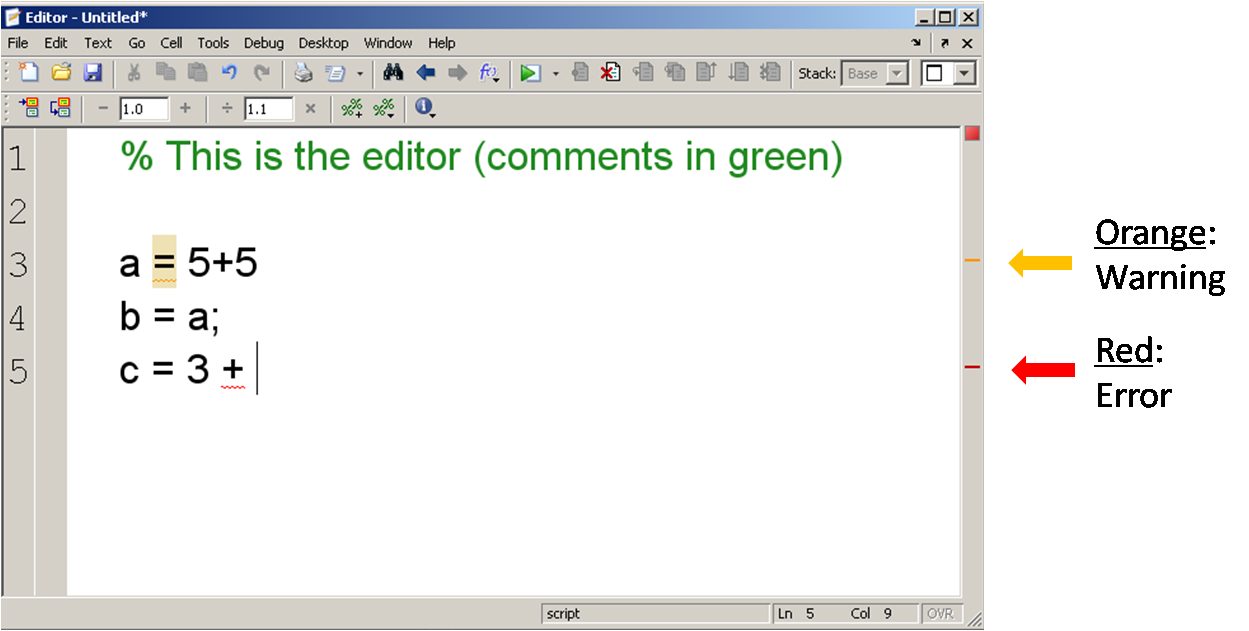
\includegraphics[scale=.9]{figures/matlab_editor}\\
%%%{\color{mygreen} hi}


%\definition{def:lineintegral}{\textbf{TITLE}}
%
%\keyidea{idea:lineintprops}{\textbf{TITLE}}
%
%\printexercises{exercises/mathcad_introduction_exercises}
